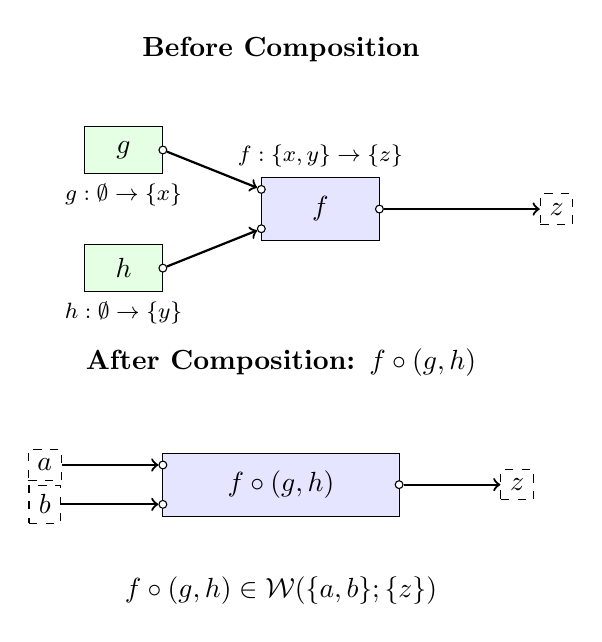
\begin{tikzpicture}[
  box/.style={rectangle, draw, minimum width=1.5cm, minimum height=0.8cm, fill=blue!10},
  subbox/.style={rectangle, draw, minimum width=1cm, minimum height=0.6cm, fill=green!10},
  wire/.style={->, thick},
  port/.style={circle, draw, fill=white, inner sep=1pt},
  interface/.style={rectangle, draw, dashed, minimum width=0.4cm, minimum height=0.25cm}
]

% Top diagram: Before composition
\node[above] at (0, 4.5) {\textbf{Before Composition}};

% Sub-operations g and h (Left side, outputs will feed into f)
\node[subbox] (g) at (-2, 3.5) {$g$};
\node[subbox] (h) at (-2, 2) {$h$};

% Main operation f (Receives outputs from g and h, centered relative to itself)
\node[box] (f) at (0.5, 2.75) {$f$};

% Output for f (Far right)
\node[interface] (out1) at (3.5, 2.75) {$z$};

% Ports for f (inputs left, output right)
\node[port] (fp1) at (-0.25, 3) {}; % Input from g
\node[port] (fp2) at (-0.25, 2.5) {}; % Input from h
\node[port] (fq) at (1.25, 2.75) {}; % Output z

% Ports for g
\node[port] (g_out) at (-1.5, 3.5) {};

% Ports for h  
\node[port] (h_out) at (-1.5, 2) {};

% Wires (Direct routing)
\draw[wire] (g_out) -- (fp1);
\draw[wire] (h_out) -- (fp2);
\draw[wire] (fq) -- (out1);

% Labels
\node[below, font=\footnotesize] at (g.south) {$g: \emptyset \to \{x\}$};
\node[below, font=\footnotesize] at (h.south) {$h: \emptyset \to \{y\}$};
\node[above, font=\footnotesize] at (f.north) {$f: \{x,y\} \to \{z\}$};

% Bottom diagram: After composition
\node[above] at (0, 0.5) {\textbf{After Composition: $f \circ (g, h)$}};

% Input interfaces for composed diagram (these are a and b)
\node[interface] (cin1) at (-3, -0.5) {$a$};
\node[interface] (cin2) at (-3, -1) {$b$};

% Composed operation box
\node[box, minimum width=3cm] (comp) at (0, -0.75) {$f \circ (g, h)$};

% Output
\node[interface] (cout) at (3, -0.75) {$z$};

% Ports
\node[port] (cp1) at (-1.5, -0.5) {};
\node[port] (cp2) at (-1.5, -1) {};
\node[port] (cq) at (1.5, -0.75) {};

% Wires  
\draw[wire] (cin1) -- (cp1);
\draw[wire] (cin2) -- (cp2);
\draw[wire] (cq) -- (cout);

% Result notation
\node[below] at (0, -1.8) {$f \circ (g, h) \in \mathcal{W}(\{a,b\}; \{z\})$};

\end{tikzpicture}